\documentclass{article}

\usepackage{graphicx}
\usepackage{tikz}
\usepackage{tikzsymbols}
\usetikzlibrary{calc,patterns,shapes.geometric}
\pagestyle{empty}
\usepackage[margin=0pt]{geometry}
\geometry{papersize={14in,12in}}

\def\centerarc[#1](#2)(#3:#4:#5){\draw[#1] ($(#2)+({#5*cos(#3)},{#5*sin(#3)})$) arc (#3:#4:#5);}

\begin{document}
	\begin{figure}
		\centering
		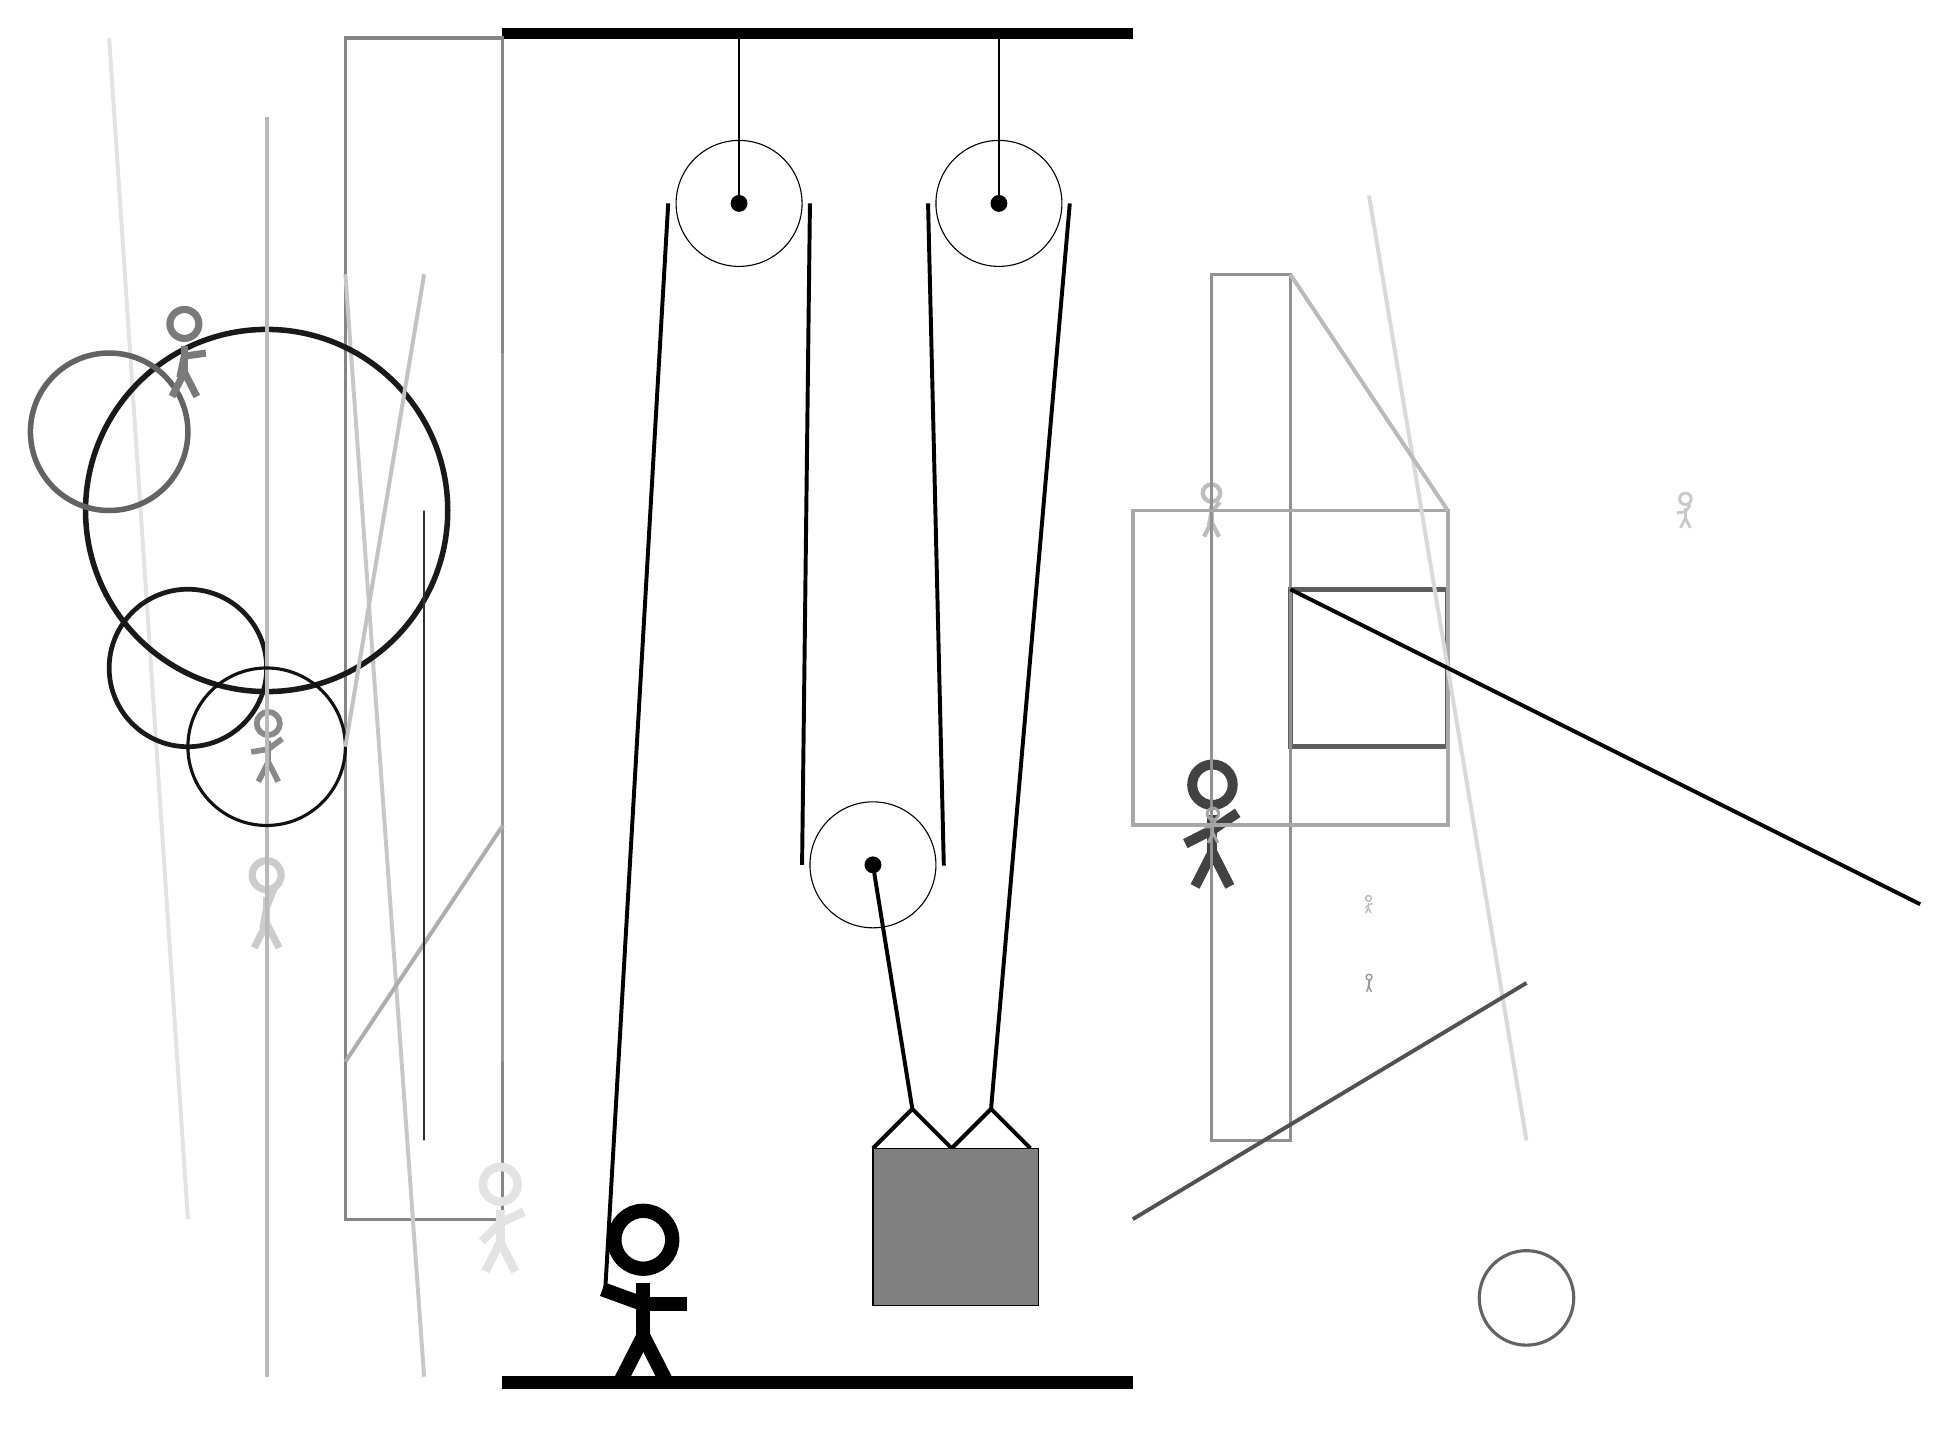
\begin{tikzpicture}
			%%%%% START %%%%%
			
			\draw[fill=black] (-2, 14) rectangle (6, 14.125);
			
			\draw (1, 11.9) circle (0.8);
			\draw[fill=black] (1, 11.9) circle (0.1);
			\draw[thick] (1, 11.9) -- (1, 14);
			
			\draw (4.3, 11.9) circle (0.8);
			\draw[fill=black] (4.3, 11.9) circle (0.1);
			\draw[thick] (4.3, 11.9) -- (4.3, 14);
			
			\draw[line width=0.5mm, color=black!11](-7, 14) -- (-6, -1);
			
			\node[line width=0.2mm, color=black!40] at (9, 2) {\Strichmaxerl[1][77][73]};
			\node[line width=0.4mm, color=black!20] at (-5, 3) {\Strichmaxerl[5][80][69]};
			\node[line width=0.5mm, color=black!74] at (7, 4) {\Strichmaxerl[7][27][34]};
			
			\draw[line width=0.4mm, color=black!48] (-2, 14) rectangle (-4, -1);
			\draw[line width=0.6mm, color=black!63] (8, 5) rectangle (10, 7);
			\draw[line width=0.5mm, color=black!22](-4, 11) -- (-3, -3);
			\node[line width=0.6mm, color=black!46] at (-5, 5) {\Strichmaxerl[4][9][37]};
			\node[line width=0.4mm, color=black!27] at (9, 3) {\Strichmaxerl[1][48][19]};
			
			\draw [line width=0.6mm, color=black!90](-6, 6) circle (1.0);
			\node[line width=0.6mm, color=black!11] at (-2, -1) {\Strichmaxerl[6][45][25]};
			\node[line width=0.4mm, color=black!21] at (13, 8) {\Strichmaxerl[2][8][55]};
			\node[line width=0.4mm, color=black!26] at (7, 8) {\Strichmaxerl[3][79][51]};
			
			\draw[line width=0.4mm, color=black!43] (7, 0) rectangle (8, 11);
			\draw[line width=0.5mm, color=black!34] (6, 8) rectangle (10, 4);
			\draw [line width=0.7mm, color=black!90](-5, 8) circle (2.3);
			
			\draw [line width=0.4mm, color=black!61](11, -2) circle (0.6);
			\draw[line width=0.5mm, color=black!27](-5, -3) -- (-5, 13);
			\draw [line width=0.4mm, color=black!93](-5, 5) circle (1.0);
			
			\draw[line width=0.4mm, color=black!40] (-2, 1) rectangle (-2, 10);
			\draw[line width=0.5mm, color=black!24](-3, 11) -- (-4, 5);
			
			\draw [line width=0.7mm, color=black!61](-7, 9) circle (1.0);
			\draw[line width=0.5mm, color=black!15](9, 12) -- (11, 0);
			\draw[line width=0.5mm, color=black!27](8, 11) -- (10, 8);
			\draw[line width=0.5mm, color=black!32](-2, 4) -- (-4, 1);
			
			\draw[line width=0.3mm, color=black!81] (-3, 8) rectangle (-3, 0);
			\draw[line width=0.5mm, color=black!68](6, -1) -- (11, 2);
			\draw[line width=0.5mm, color=black!100](8, 7) -- (16, 3);
			\node[line width=0.2mm, color=black!36] at (7, 4) {\Strichmaxerl[2][3][70]};
			
			\node[line width=0.7mm, color=black!52] at (-6, 10) {\Strichmaxerl[5][78][8]};
			
			\draw (2.7, 3.5) circle (0.8);
			\draw[fill=black] (2.7, 3.5) circle (0.1);
			
			\draw[line width=0.5mm]  (2.7, -0.1) -- (3.2, 0.4) -- (3.7, -0.1) -- (4.2, 0.4) -- (4.7, -0.1);
			\draw[fill=black!50] (2.7, -0.1) rectangle (4.8, -2.1);
			
			\draw[line width=0.5mm](-0.7, -1.9) -- (0.1, 11.9);
			\centerarc[line width=0.5mm](1, 11.9)(0:180:0.9);
			\draw[line width=0.5mm](1.9, 11.9) -- (1.8, 3.5);
			\centerarc[line width=0.5mm](2.7, 3.5)(180:370:0.9);
			\draw[line width=0.5mm] (3.6, 3.49) -- (3.4, 11.9);
			\centerarc[line width=0.5mm](4.3, 11.9)(0:180:0.9);
			\draw[line width=0.5mm](4.2, 0.4) -- (5.2, 11.9);
			\draw[line width=0.5mm] (3.2, 0.4) -- (2.7, 3.5);
			
			\node at (-0.2, -2) {\Strichmaxerl[10][-20][0]};
			
			\draw[fill=black] (-2, -3) rectangle (6, -3.15);
			
			%%%%% END %%%%%
		\end{tikzpicture}
	\end{figure}	
\end{document}